\chapter{Introduction}
\section{Course Structure and Logistics}
\begin{minipage}{.3\textwidth}
    \begin{center}
        \begin{tikzpicture}
        \clip (0,0)  circle (2cm) ;
        \node[anchor=center] at (0,-0.5) {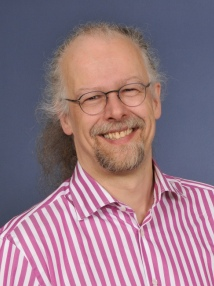
\includegraphics[width=4.5cm]{introduction/images/paul_kelly.jpg}}; 
        \end{tikzpicture}
        \centerline{\textbf{Prof Paul Kelly}}
    \end{center}    
\end{minipage}
\hfill
\begin{minipage}{.68\textwidth}
    Teaching the entire course.
    \begin{itemize}
        \item Microprocessor design.
        \item Optimising software for hardware, and compiler design.
        \item Optimising hardware for specific software tasks.
        \item Challenges past, present \& future.
    \end{itemize}
    Taught through pre-recorded lectures and live tutorial sessions.
\end{minipage}
\\ \begin{minipage}{.63\textwidth}
    This course is largely textbook based.
    \begin{itemize}
        \item $936$ pages covering the course content and more.
        \item Useful appendices covering both introductory and advanced material.
    \end{itemize}
    The book is written by John Hennessy and David Patterson.
\end{minipage}
\hfill
\begin{minipage}{.35\textwidth}
    \begin{center}
        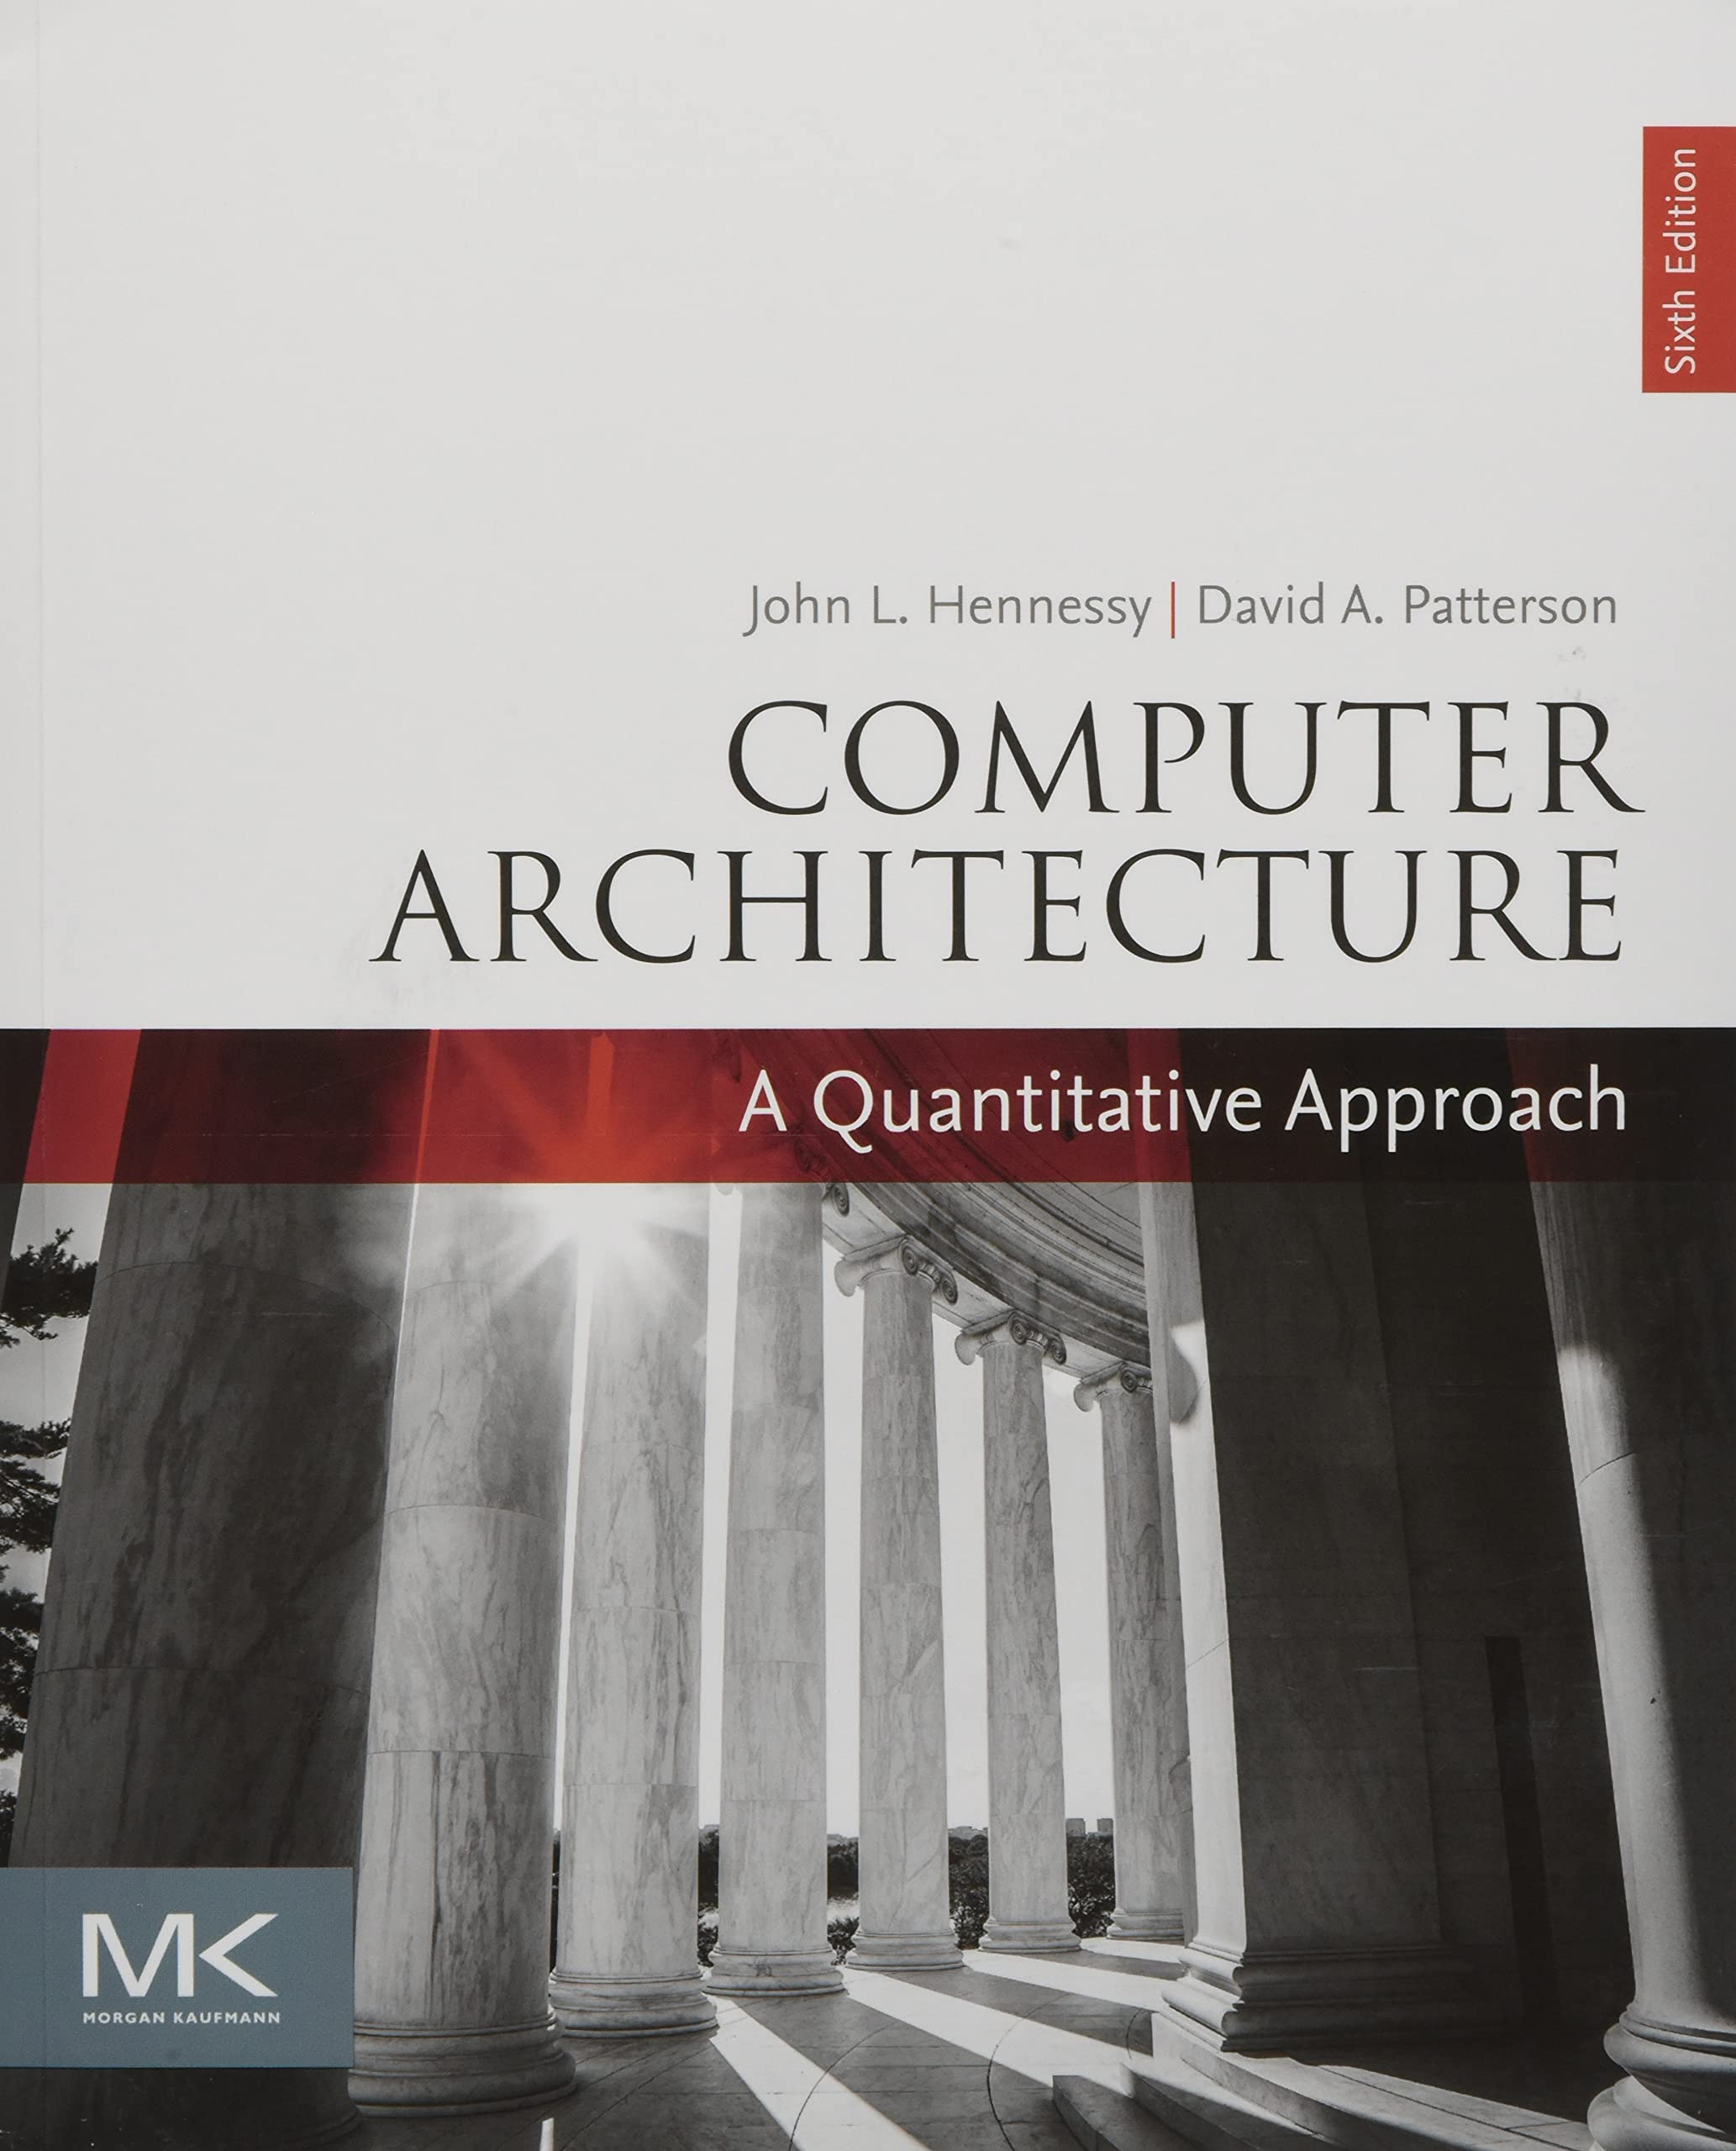
\includegraphics[height=6cm]{introduction/images/comp_arch_quant_approach.jpg}
    \end{center}
    \centerline{\textbf{Computer Architecture:}}
    \centerline{\textbf{A Quantitative Approach (\nth{6} Edition)}}
\end{minipage}

\lectlink{https://imperial.cloud.panopto.eu/Panopto/Pages/Viewer.aspx?id=9c34ae74-31d9-4a8b-89cd-af2a010ddb5d}{Chapter 1 - Part 1: Introduction}